\documentclass{article}
\usepackage{graphicx} % Required for inserting images
\usepackage[
    backend=biber,
    style=numeric,
]{biblatex}
\usepackage{url}

\addbibresource{bibfile.bib}

\title{HCS502: Assessment \- AI/ML Project \- 2310190}
\author{Thomas Morton}
\date{June 2025}

\begin{document}

\maketitle

\begin{abstract}
This study aims to explore and employ machine learning techniques in order to predict the cost of insurance premiums for an individual based on details about the driver as well as information about the vehicle. The research will also outline how each of these features affects the insurance premium for a driver. The data set being used has 1000 records containing the aforementioned data. This dataset will be used to train and analyse both simple and multivariate regression models, clustering algorithms and neural networks. Data preprocessing was carried out on the data, which consisted of normalisation in the form of scaling and anomaly identification.

\end{abstract}

\newpage

\section{Introduction}
Car insurance and its workings are a mystery to many. It traditionally relies on analysis and experts in the domain of car insurance to make assumption and asses the risk of certain drivers and vehicles and set a driver's insurance premium based on this knowledge and experience. In the modern world, with comparison sites and insurers in the 100's or even 1000's, artificial intelligence (AI), along with machine learning (ML), probably already run the business side of most insurers on the market. Although it may seem unfair to let these algorithms control the prices, they use data-driven methods which is trained on raw facts from the world of motoring. This technology offers an automated solution, saving the companies a lot of money in training individual staff members on the risk factors to look out for in a person. 

This project investigates how effective a simple regression algorithm, using one factor, or a multivariate algorithm, using multiple factors, can be used to predict car insurance premiums based on the information provided. Linear regression is known for its interpretability and efficiency in a computational sense\cite{scikit_LR}, which allows for easy identification of trends and displaying the correlation between key factors. In applying these models to a structured dataset, this study aims to explore how effectively insurance premiums can be predicted, which will allow the assessment of the model accuracy and evaluate how this can also present the risk of over-fitting to the data.

Understanding the relationship between these factors is imperative to the research into the workings of insurance company pricing structures. This research seeks to provide more transparent pricing and show the factors that have the biggest impact on an insurance policy.

\newpage
\section{Dataset and Pre-processing}

\begin{figure}[h]
\centering
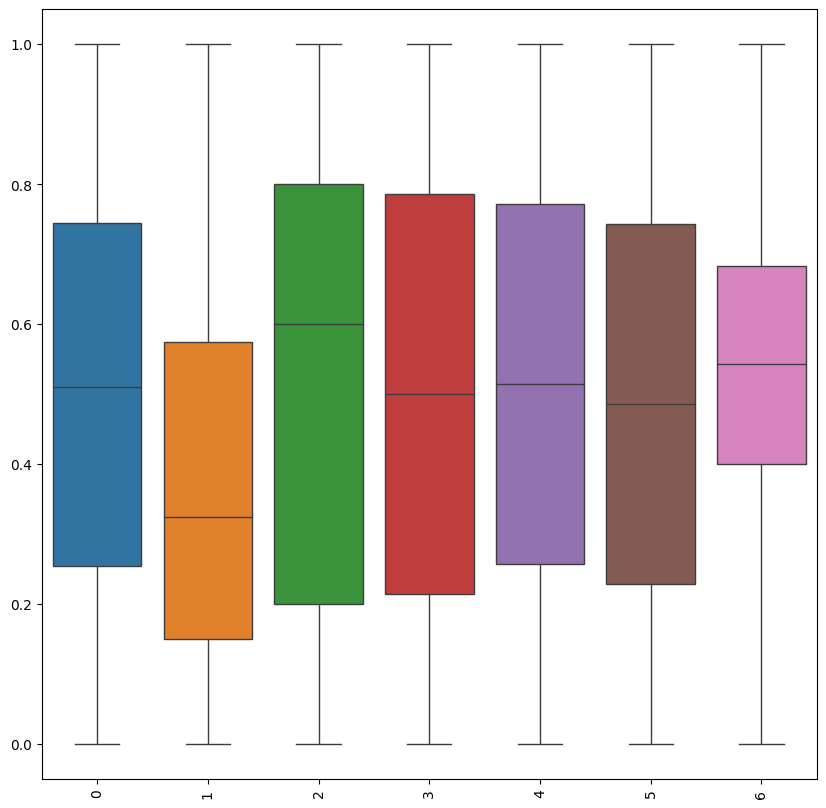
\includegraphics[width=0.8\textwidth]{boxplot.png}
\caption{Boxplot of Normalised Variables}\label{fig:boxplot}
\end{figure}

The dataset was sources from Kaggle.com and provides an array of information including the details about a driver, their vehicle and the insurance premium they were quoted because of this\cite{Sriram_2025}. The dataset consists of 1000 rows of data containing numerical features along with the insurance price. Thee features include; Driver Age, Driver Experience, Previous Accidents, Annual Mileage (KM), Car Manufacturing Year, Car Age and finally, the taget variable, Insurance Premium in US dollars.  

To ensure the data was of a high enough quality, there was some initial exploratory analysis that took place in the form of normalisation, box plots and statistical summary. The inital check was to make sure where were no null values in the data, of which there are none as shown below in the output of an `isnull().sum()' check.

\begin{verbatim}
Driver Age                   0
Driver Experience            0
Previous Accidents           0
Annual Mileage (x1000 km)    0
Car Manufacturing Year       0
Car Age                      0
Insurance Premium ($)        0
dtype: int64
\end{verbatim}





\newpage
\section{Exploratory Data Analysis (EDA)}

\begin{figure}[h]
\centering
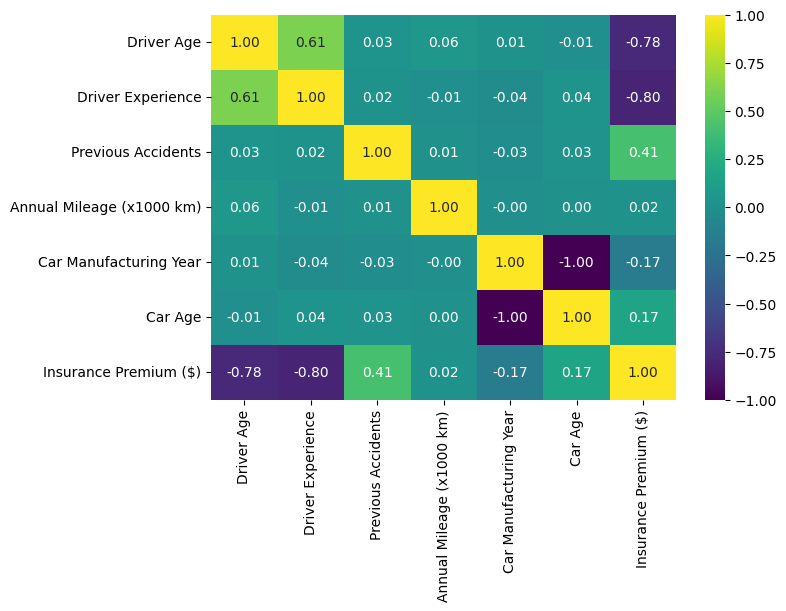
\includegraphics[width=0.8\textwidth]{heatmap.png}
\caption{Correlation Heatmap of All Features}\label{fig:heatmap}
\end{figure}

\newpage
\section{Modelling and Evaluation}

Linear regression models aim to establish a linear relationship between input features $x_i$ and the continuous target variable $y$ (insurance premium), typically expressed as:

$$
\hat{y} = \beta_0 + \sum_{i=1}^p \beta_i x_i
$$

where $\beta_0$ is the intercept and $\beta_i$ are the coefficients learned from data\cite{hastie_09_elements-of.statistical-learning}.



\begin{figure}[h]
\centering
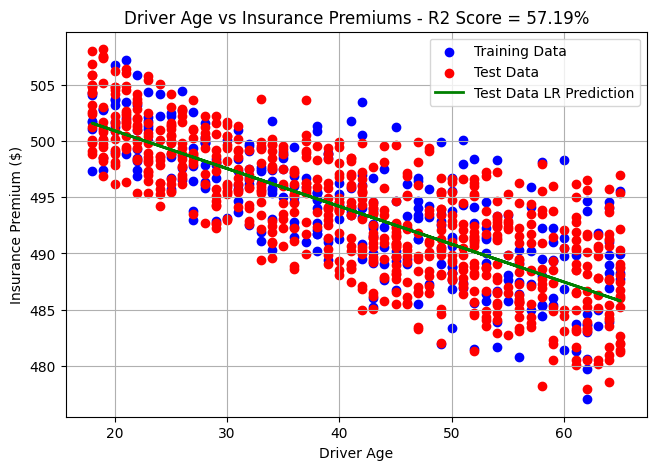
\includegraphics[width=0.8\textwidth]{age_insurance_LR.png}
\caption{Regression Line: Driver Age vs Insurance Premium}\label{fig:regression_age}
\end{figure}

\begin{figure}[h]
\centering
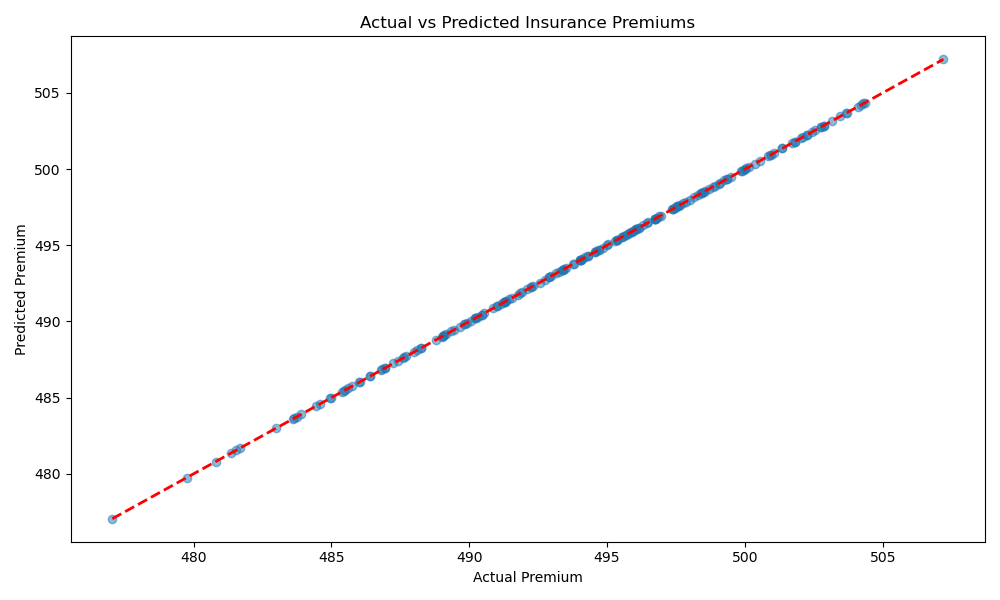
\includegraphics[width=0.8\textwidth]{actual_vs_predicted.png}
\caption{Actual vs Predicted Premiums (Multivariate Model)}\label{fig:multivariate_regression}
\end{figure}

\subsection{Model Comparison}

\begin{itemize}
\item Simple linear regression provides interpretability but lower accuracy.
\item Multivariate regression achieves high performance on synthetic data but raises questions about generalizability.
\item Further work may include Ridge/Lasso regression to assess generalisation.
\end{itemize}

\newpage
\section{Software Environment}


\section{Software Environment}

The machine learning pipeline was implemented in Python 3.13.2 using popular scientific libraries including \texttt{pandas} for data manipulation, \texttt{scikit-learn} for modeling, and \texttt{matplotlib} and \texttt{seaborn} for visualization.



\newpage
\section{Results Analysis}

\newpage
\section{Ethical Considerations}

The use of machine learning for predicting car insurance premiums introduces several ethical concerns:

\textbf{Fairness and Bias:} 

\textbf{Data Privacy:} 

\textbf{Transparency:} 

\textbf{Accountability:} 

\newpage
\section{Conclusion}

\newpage

\printbibliography

\end{document}
